% !TEX program = XeLaTeX
% !TEX encoding = UTF-8
\documentclass[UTF8,nofonts]{article}
%{ctexart}


%\setCJKmainfont[BoldFont=FandolSong-Bold.otf,ItalicFont=FandolKai-Regular.otf]{FandolSong-Regular.otf}
%\setCJKsansfont[BoldFont=FandolHei-Bold.otf]{FandolHei-Regular.otf}
%\setCJKmonofont{FandolFang-Regular.otf}

\usepackage{url}
\usepackage{cancel}
\usepackage{xspace}
\usepackage{graphicx}
\usepackage{multicol}
\usepackage{multirow}
\usepackage{subfig}
\usepackage{amsmath}
\usepackage{amssymb}
%\usepackage[a4paper, width=180mm, top=18mm, bottom=22mm, includeheadfoot]{geometry}
\usepackage[a4paper, width=140mm, top=18mm, bottom=22mm, includeheadfoot]{geometry}
\usepackage{booktabs}
\usepackage{array}
\usepackage{verbatim}
\usepackage{caption}
%\usepackage{natbib}
\usepackage{booktabs}
\usepackage{float}
\usepackage{pdflscape}
\usepackage{mathtools}
\usepackage[usenames, dvipsnames]{xcolor}
\usepackage{afterpage}
\usepackage{pgf}
\usepackage{tikz}
\usepackage{dirtree}
\usepackage{amsfonts}
\usepackage{tkz-graph}


\newtheorem{definition}{Definition}[section]
\newtheorem{theorem}{Theorem}[section]
\newtheorem{lemma}{Lemma}
\newtheorem{proof}{Proof} [section]



\usepackage[toc, page, title, titletoc, header]{appendix}
\usepackage{marginnote}
\usepackage{tablefootnote}

%\renewcommand\appendixname{附\ 录}
%\renewcommand\appendixpagename{附\ 录}
%\renewcommand\appendixtocname{附\ 录}
\renewcommand\abstractname{Abstract}


\usepackage{perpage} %the perpage package
\MakePerPage{footnote} %the perpage package command

\usetikzlibrary{shapes.geometric}%
\usepackage{color}
%\usepackage[pages=some, placement=top]{background}
\usepackage{eso-pic}

\title{\textbf{LOOPRING}\\\textbf{Decentralized Token Exchange Protocol}\\\textbf{A simplified version}\\v1.4}
\author{
  daniel@loopring.org\\
  jay@loopring.org\\
  Thomas Tabbaza from our community\\
  \\
  \textit{Loopring Project Ltd}\\
%  \textit{http://Loopring.io}\\
  \textit{foundation@loopring.org}\\
 }

\makeatletter
\def\CTEX@section@format{\Large\bfseries}
\makeatother

\makeatletter
\newenvironment{tablehere}
 {\def\@captype{table}}
 {}

\newenvironment{figurehere}
 {\def\@captype{figure}}
 {}
\makeatother
%
%\newcommand\BackgroundPic{%
%\put(0, 0){%
%\parbox[b][\paperheight]{\paperwidth}{%
%\vfill
%\centering
%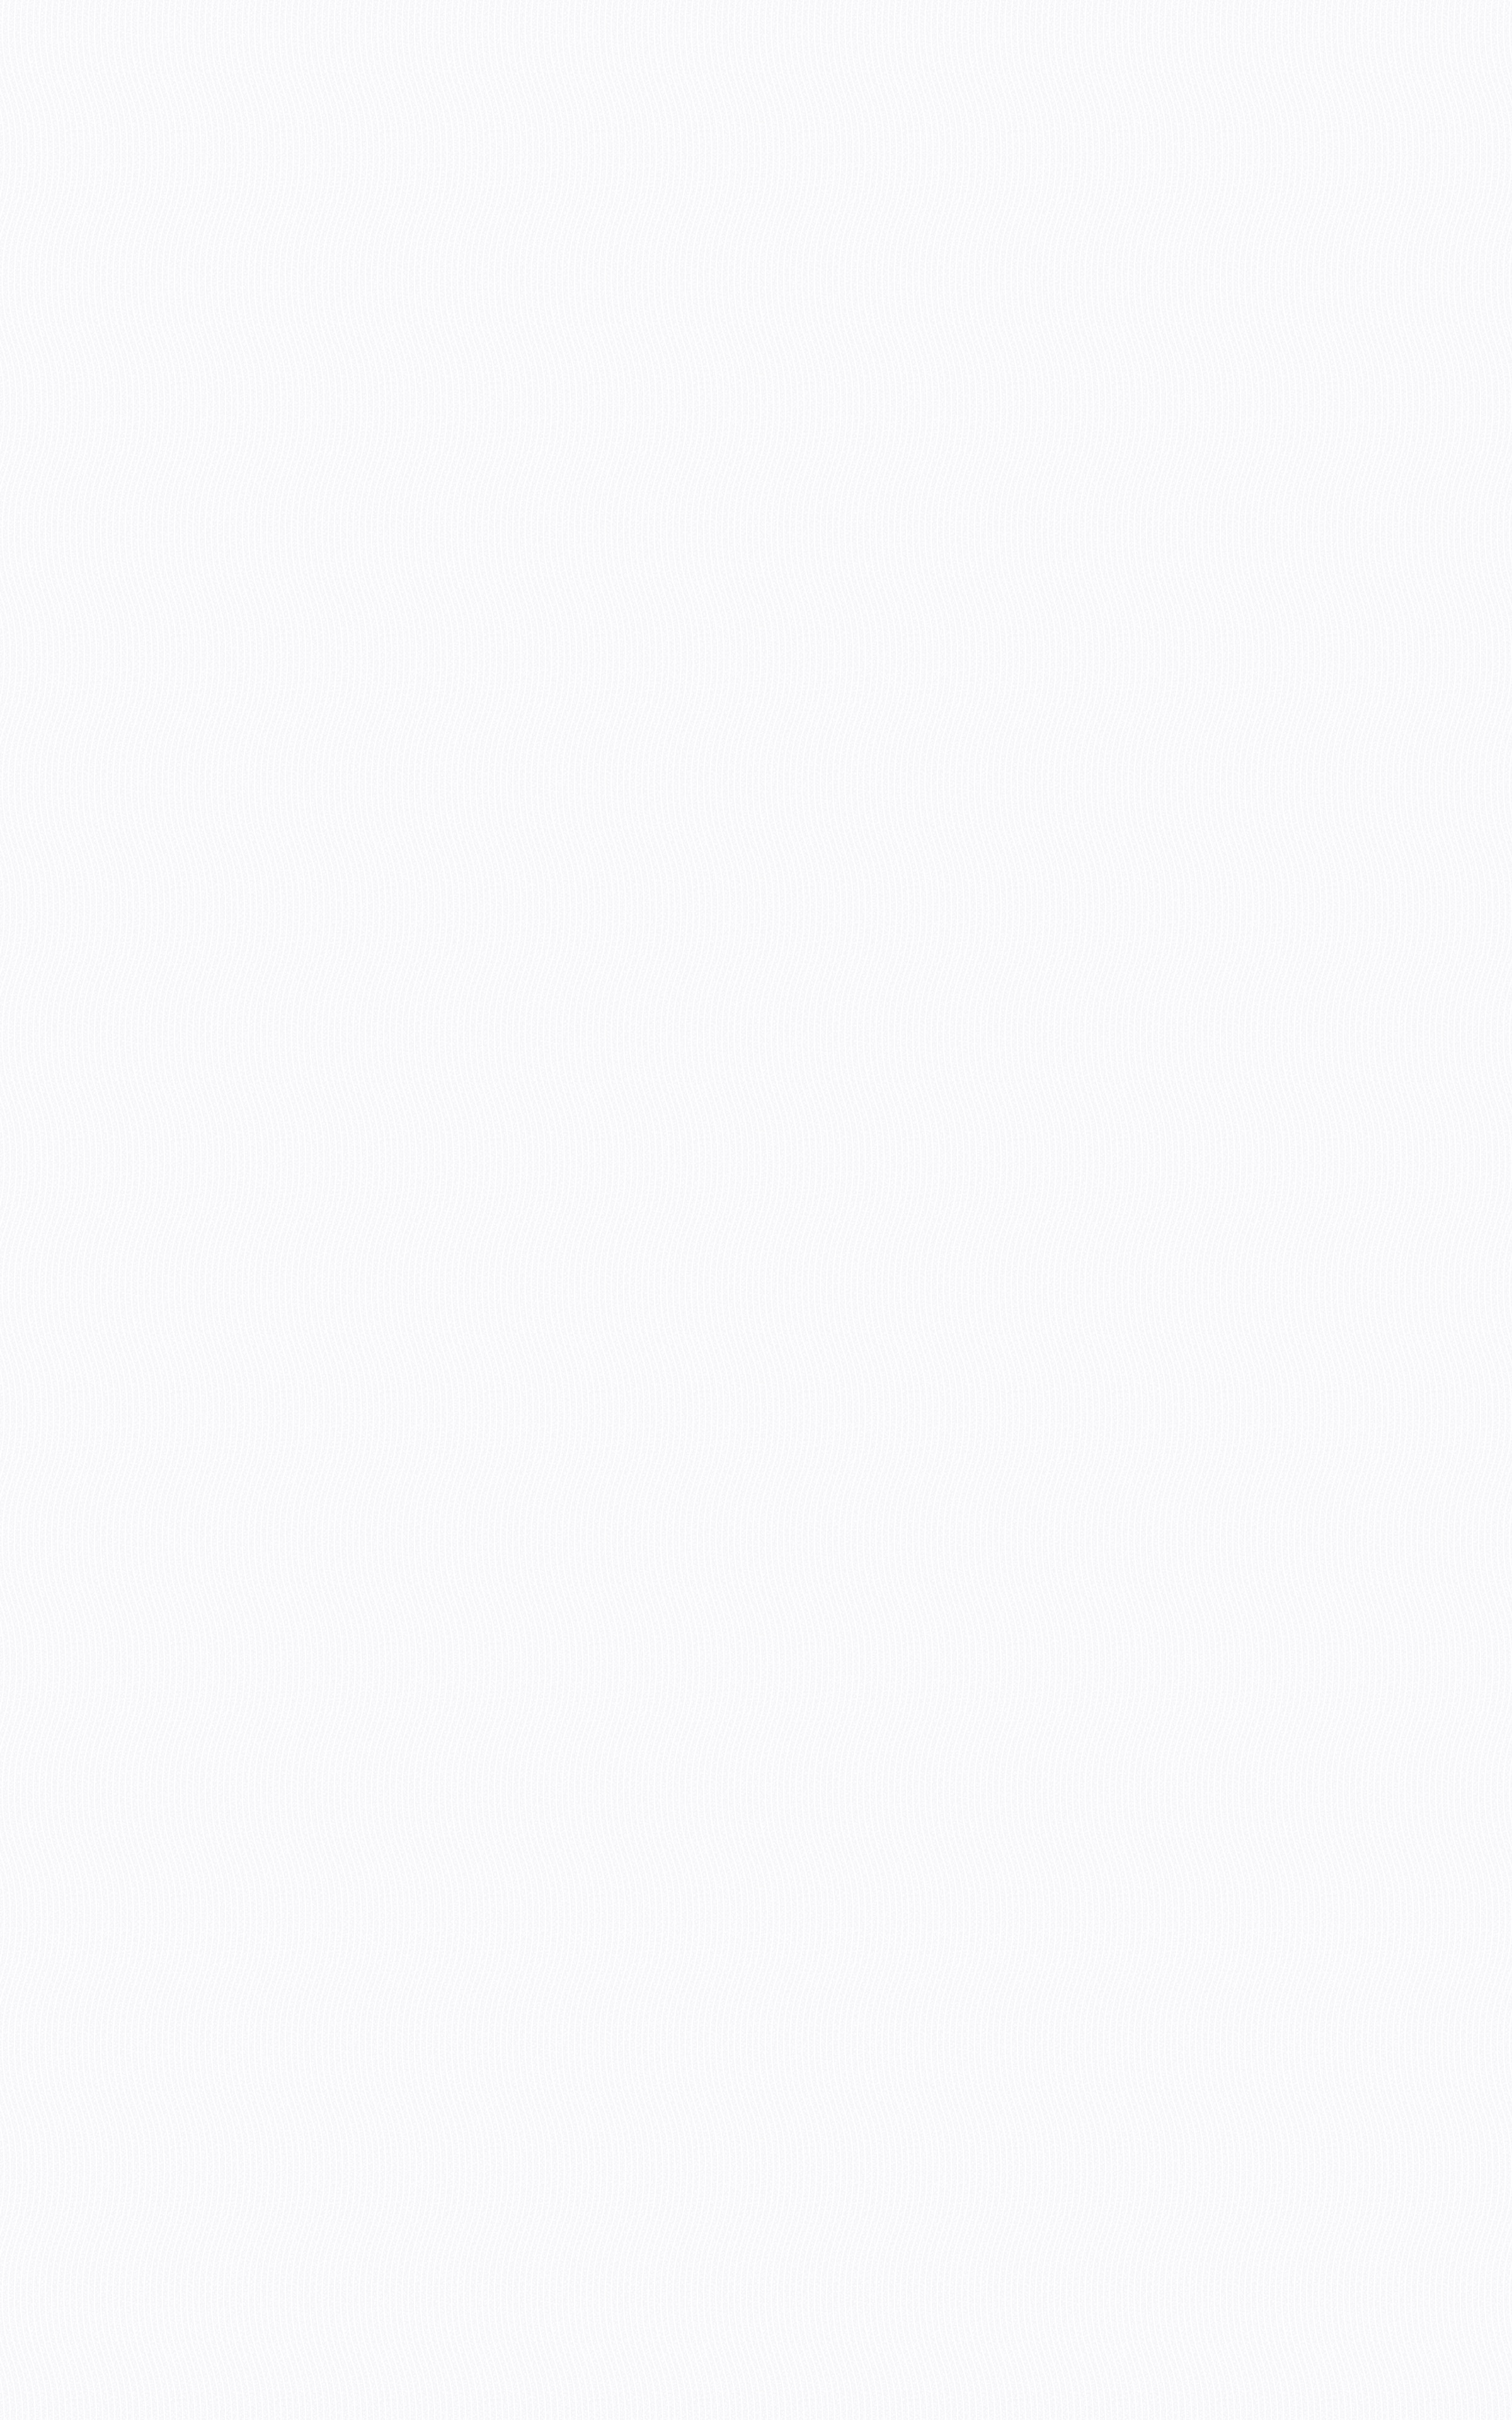
\includegraphics[width=\paperwidth, height=\paperheight, %
%%keepaspectratio]{images/background.jpg}%
%]{images/background.jpg}%
%\vfill
%}}}


\begin{document}
%\AddToShipoutPicture{\BackgroundPic}
\maketitle


\section{Overview\label{sec: overview}}

Loopring is a decentralized exchange protocol for ERC20 Tokens. However, Loopring is not an exchange per se. The building blocks of a traditional centralized exchange are disassembled and reassembled again with different roles to fit the decentralized environment. These roles include, but are not limited to, wallet, relays, order books, browsers, ring-miners, and asset tokenization services.

At the outset, Ethereum will serve as the first public blockchain supported by Loopring. Moving forward, other blockchains with smart contract capability, such as NEO, Qtum, and EOS, can also be supported in a similar way.

An Ethereum smart-contract is at the core of the Loopring decentralized exchange system. Loopring’s system design allows for several improvements over traditional centralized exchanges, such as:

\begin{itemize}
 \item Reduced counterparty and exchange risk: The tokens stay in the user's wallet and are never locked by orders.
 \item High liquidity: Ring-matched orders provide increased liquidity on any trading pair.
 \item Fairness: Loopring’s fee and discount model allows for fairness between all parties involved (Makers, Takers, Exchanges, and Miners).
 \item No reliance on a centralized authority: The whole system is completely decentralized.
\end{itemize}


\section{Ecosystem\label{sec: ecosystem}}

This section introduces key parts of the Loopring ecosystem and how they interact with each other. These key parts jointly provide all of the same functionalities a centralized exchange offers.
\begin{itemize}


\item \textbf{Wallets}
A common wallet service/interface that gives users access to their tokens and provides users with a way to send orders to the Loopring network.

\item \textbf{Ring Miners}
Ring-miners determine the most efficient method to fulfill received orders through ring-matching. The process is computational heavy and conducted completely off-chain. The process produces chains of trades involving at least two tokens, which we call an order ring.

\item \textbf{Loopring Protocol Smart Contracts}
A set of smart contracts that check ring-matched orders received from miners, performs the token transfers on behalf of users, incentivizes miners, and emits events. The relay/order browsers monitor these events to keep their order books and trade history up to date.

\item \textbf{Relays}
Relays maintain public order books and trade history, and broadcast new orders to other relays and ring-miners.

\item \textbf{Asset Tokenization Services}
Asset tokenization services act as a bridge between assets that cannot be directly traded on Loopring. They are centralized services run by trustworthy companies or organizations. A user can deposit his assets (fiat or tokens from other chains) and get tokens issued. The user reclaims his deposit by returning Loopring’s LRC tokens. LRC is not a cross-chain exchange protocol, but the Asset Tokenization Service makes it possible to trade Ethereum ERC20 tokens with physical assets as well as assets on other blockchains. However, Asset Tokenization Services is not part of Loopring project.
\end{itemize}

\section{Lifecycle of a Successful Order on the Loopring Network}

\begin{center}
\begin{figurehere}
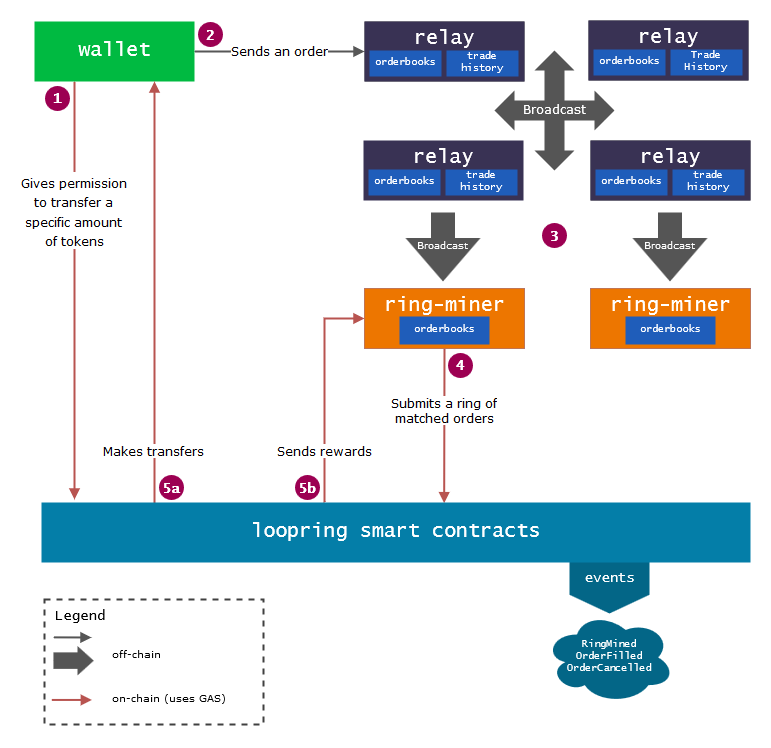
\includegraphics[height=12cm]{images/loopring-overview.png}
\label{fig: Loopringrotocol}
\end{figurehere}
\end{center}

\begin{enumerate}
 \item \textbf{The user wants to make a trade}: The user wants to exchange X amount of TokenA for Y amount of TokenB. The current rate and order book for this pair can be found on multiple sources provided by the relays or any other interface hooked up to the network (e.g. order book browsers). Once a user is ready, he uses his wallet interface to enter the details of his order and submits the order. An amount of LRC can be added to the order as a fee for miners. Orders with a higher LRC fee have a better chance to be processed earlier by miners.
 \item \textbf{ERC20 authorization}: The wallet authorizes the Loopring smart contracts to handle X amount of TokenA the user wants to sell. This authorization does not lock the user's tokens. The user retains the freedom to move tokens while the order is being processed by the network. If the sender's wallet balance is being checked at some point (by a miner or the Loopring) and the remaining funds are insufficient, it will be considered scaled-down. A scaled-down order is not the same as a cancelled order – a scaled-down order will be automatically scaled up to its original size if sufficient funds are deposited to its address. Cancellation is a one-way manual operation and cannot be reverted.
 \item \textbf{Sending the order to the network}:Once the authorization is made, the order data is signed with the sender’s private key. Next, the wallet sends the order along with its signature to one or more nodes in the network (relay or ring-miner).
 \item \textbf{Broadcast}: On the order’s reception, relays update their public order book and broadcasts the order to other relays as well as ring-miners to start the order processing as quickly as possible.
 \item \textbf{Order matching}: Ring-miners receive the order and add it to their order book. Each one of them tries to fulfill the order or partially fill it at the given exchange rate or a better rate by ring-matching the order with multiple other orders. Ring-matching is the main reason why the protocol is able to provide increased liquidity over any pair. If the rate is better than the rate the user asked for, the savings are shared amongst all the orders in the ring - this is called a margin split. As the processing fee, the miner can either claim the margin split and return the LRC back to the user or retain the LRC fee.
 \item \textbf{Validation and settlement}: The ring is received by the Loopring protocol contract. It makes multiple checks to verify the miner's supplied data to determine if the ring can be settled fully or partially (depending on the fill rate of the orders in the ring and the tokens in the user’s wallets). If all checks are successful, the contract transfers the token to the users (5a) and pays the miner's fees (5b) at the same time. This operation is atomic.
\end{enumerate}

\section{Issues with Centralized Exchanges}

To better understand the need for Loopring, we first need to address the issues with regard to a centralized exchange model.

The Figure below illustrates a very simplified view of what happens when users send their tokens to a centralized exchange.


\begin{center}
\begin{figurehere}
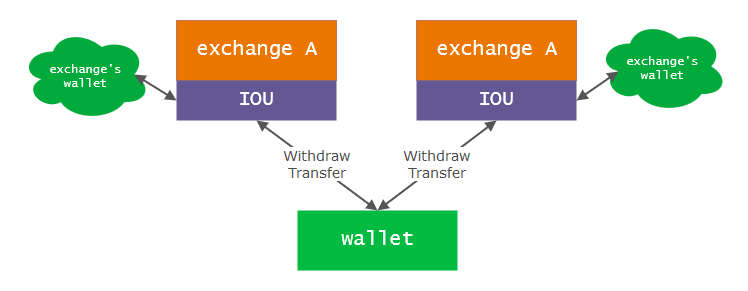
\includegraphics[height=4cm]{images/centralized-model.png}
\label{fig: Loopringrotocol}
\end{figurehere}
\end{center}

Users will first have to deposit their tokens in the exchange in order to use the exchange to trade their tokens. Users’ tokens are then sent to the exchange's wallet, and the exchange gives them back an IOU, which represents a proof of debt. Next, users trade their IOU with other users’ IOUs. Finally, when users want to withdraw, they return the IOU to the exchange, which then sends the tokens back to the users’ external wallet address.

\begin{itemize}

 \item \textbf{Lack of Security} In this model, users do not have control over their tokens. It allows for instant transactions on the exchange, albeit, while carrying a lot of risk. There are multiple scenarios in which users can lose their money due to centralized exchange custodial risk (frozen account, exchange shutting down, hacking, developer's mistakes, etc.).

 \item \textbf{Lack of Transparency}
Anything can happen to users’ tokens when they are held in exchange wallets. It is always too late when an exchange becomes insolvent without any notice to the user.

 \item \textbf{Lack of Liquidity}
Users are only able to trade within the exchange’s own order pool and supported token pairs. If there is not enough volume users can try trading on another exchange. If, however, the token pair that the users wants to trade is not supported, users can try making indirect trades with other pairs or transfer their funds to another exchange. Either way users get hit with multiple fees and will likely lose asset value.
\end{itemize}

\section{Loopring Smart Contract}
The Loopring Smart Contracts (LSC) are a set of Ethereum contracts that implement the Loopring protocol. The code is open source available on github.


\subsection{Management of Orders}

To understand what LSC does, we must first take a look at the anatomy of an order, the available actions for the user, and how the current order state is tracked.
\subsubsection{Anatomy of an Order}

An order is a pack of data that describes the user’s market intent . To ensure the origin of the order, it is signed against the hash of its parameters with the user's private key. The signature is sent along with the order data on the network. This requires the order to stay immutable during its lifetime to verify the sender's address.


\begin{equation}
Signature = ECDSA(SHA3(order_params))
\end{equation}

Even if the order never changes, LSC has the possibility to compute its current state.

Relevant variables of an order's parameters (for a complete list of order parameters, take a look at the following codes):

\begin{table}[hbt]
 \centering
\begin{tabular}{p{4cm}|p{10cm}} %设置了每一列的宽度, 强制转换.
owner & The owner (signer) address\%\\
\hline
tokenS & Token to sell\\
\hline
tokenB & Token to buy\\
\hline
amountS & Amount of tokenS to sell\\
\hline
amountB &Amount of tokenS to buy\\
\hline
buyNoMoreThanAmountB &See below\\
\hline
ttl &Seconds after which the order will expire (time to live)\\
\hline
lrcFee &Max amount of LRC to pay to the miner\\
\hline
marginSplitPercentage & The percentage of margin paid to the miner (when a better rate is found)\\
 \end{tabular}
\end{table}



The model shown above is described as an Unidirectional Order Model (UDOM).The exchange rate r of the order is determined using the following formula r = amountS/ amountB. When a miner performs ring-matching, there is a possibility that the miner finds the user a better rate that gets the user more tokenB than the amountB the user specified. But, if the buyNoMoreThanAmountB flag is set, the LSC will make sure the user still receives exactly amountB of tokenB.

Example: with $amountS = 10$ and $amountB = 2$, $r = 10/2 = 5$. This means that the user is willing to sell 5 tokenS for each tokenB. The miner performs ring-matching and finds the user a rate of 4, topping the amount the miner could get the user to 2.5 tokensB instead of 2. The user only wanted 2 tokensB and set the buyNoMoreThanAmountB flag to true. The LSC takes that into consideration and still performs the transaction at a rate of 4 and the user ended up selling 4 tokenS for each tokenB, effectively saving 2 tokenS. Keep in mind that this does not take into account the miner’s fees.

\subsubsection{Full or Partial Cancellation}
A user can partially or fully cancel an order by sending a special transaction to the LSC, containing the order’s details and the amounts to cancel. The LSC will take that into account, store the amounts to cancel, and emit an OrderCancelled event to the network.

\subsubsection{Fill and Cancellation Tracking}
The LSC keeps track of fill and cancellation amounts by storing their values using the order's hash as an identifier. This data is publicly accessible and OrderCancelled /OrderFilled events are emitted when it changes.
This tracking is useful for the LSC during the ring settlement step.

\subsection{Verification of Miner Supplied Data}

This section will talk about what the LSC expects to receive from the miners and the steps taken to verify the data.

\subsubsection{Order Ring}
The LSC expects to receive order rings from the miners. An order ring is multiple orders linked together in a way that allows them to be all matched at their desired exchange rate or better. The diagram below illustrates an example.
\begin{center}
\begin{figurehere}
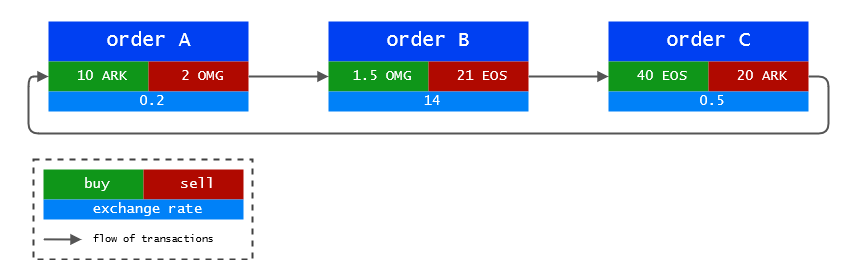
\includegraphics[height=4cm]{images/order-ring.png}
\label{fig: Loopringrotocol}
\end{figurehere}
\end{center}

Notice how each order's token to sell is the following order's token to buy. It creates a loop that allows each order to effectively sell and buy its desired tokens without having a matching order of the opposite pair.
A ring is said to be valid when all the transactions can be made at an exchange rate equal or better than the original one specified by the user. To verify the ring validity, the product of the original exchange rates of all orders should be equal to or greater than 1.
Example: Let's check if the above ring in the diagram is valid. $0.2 * 14 * 0.5 = 1.4$ the result is greater than 1, thus the trade should be possible.

\subsubsection{Order Ring Validation}

The LSC does not perform the exchange rate or amount calculations, but it still has to verify what the miner supplied for these values. Miners do this for two main reasons: solidity does not have support for floating point maths, especially $pow(x, 1/n)$, and it is desired that the computation is made off-chain to save gas.


\subsubsection{Sub-Loop Checking}
This step prevents covered interest arbitrage. Once a miner finds a valid ring, the miner could be tempted to add other orders to it to achieve a zero-risk covered interest arbitrage. This is considered unfair conduct for a miner in Loopring.
The diagram bellow illustrates the previous valid ring where two orders were added.
\begin{center}
\begin{figurehere}
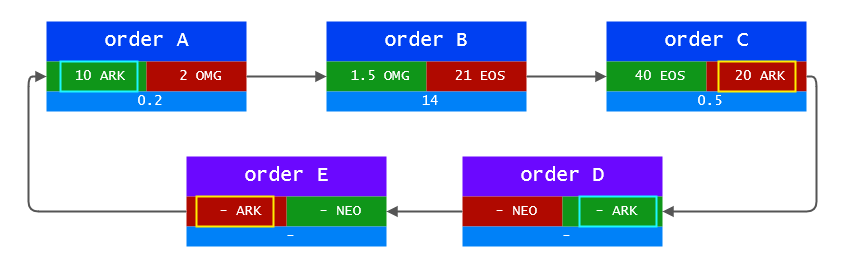
\includegraphics[height=4cm]{images/order-ring-sub-loop.png}
\label{fig: Loopringrotocol}
\end{figurehere}
\end{center}
To prevent this, Loopring requires that a valid loop cannot contain a sub-loop. There is a very simple way to check this: a token cannot be twice in a buy or sell position. In the above diagram, we can see that ARK is twice as a token to sell and twice as a token to buy.

\subsubsection{Fill Rate Checking}

For the reasons stated above, miners calculate the rate of transactions in the ring. Therefore, the LSC must verify that the calculation is correct.
First, this verifies that the sell rate the miner supplied for each order is at least less than or equal to the original sell rate set by the user. This means that the user receives at least the exchange rate requested or a better rate at the moment of the transaction.
Next, to ensure fairness, once the exchange rates are confirmed we make sure that all the margins (discounts) are the same percentage.

\subsubsection{Order Scaling}
Once the fill rates are verified, orders are scaled according to: the history of filled and cancelled amounts, and the current balance of the sender’s accounts
Order scaling finds the order with the smallest amount to be filled according to the above characteristics, and uses it as a reference for scaling all the transactions in the ring.
Example: If the smallest amount to be filled compared to the original order is 5\%, all the transactions in the ring are scaled down to 5\%. Once the transactions are completed, the order that was considered to have the smallest amount remaining (to be filled) should be completely filled.

\subsection{Ring Settlement}
If all the lights are green from the previous checks, the transactions can be made.
\subsubsection{Transactions}
To make the transactions, LSC uses the \textbf{TokenTransferDelegate} smart contract (delegate). The introduction of such a delegate makes upgrading the protocol’s smart contract easier because all orders only need to authorize this delegate instead of all the different versions of the protocol.
For each order in the ring, a payment of tokenS is made to the previous order. Then the miner's fee is paid depending on what fee model the miner chooses. If the model was the LRC fee, the remaining amount after the fee is paid is returned to the order's owner. Finally, an \textbf{OrderFilled} event is recorded.
Once all the transactions are made, a \textbf{RingMined} event is recorded.
\subsubsection{Fee Model}

This section describes Loopring’s current fee model.
In the current fee model, the miner has two possible options. When a user creates the order, the user specifies a maximum of LRC to be paid to the miner as a fee, as well as a percentage of the margin made on the order that the miner can claim. This is called the margin split. The miner may select either choice.
A representation of the margin split:
\begin{center}
\begin{figurehere}
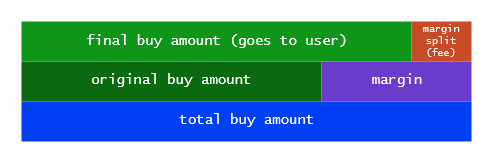
\includegraphics[height=4cm]{images/margin-split.png}
\label{fig: Loopringrotocol}
\end{figurehere}
\end{center}

If the miner decides that the margin on the ring is too small, the miner will choose the LRC fee. On the contrary, if the margin is enough for the resulting margin split to be worth more than the LRC fee, the miner will choose the margin split.
But there is a twist: when the miner chooses the margin split, the miner has to pay the user a fee, which is equal to what the user would have paid as a fee to the miner for the transaction. This increases the threshold where the miner will choose the margin split to twice the LRC fee of the order, adding weight to the LRC fee choice.
From the miner's point of view, this allows the miner to receive a constant income on low- margin rings with the drawback of getting less income from the larger margin rings. As the market grows and becomes more mature, we expect to have less high-margin rings. Loopring’s fee model is based on that future.
We end up with the following graph:
\begin{center}
\begin{figurehere}
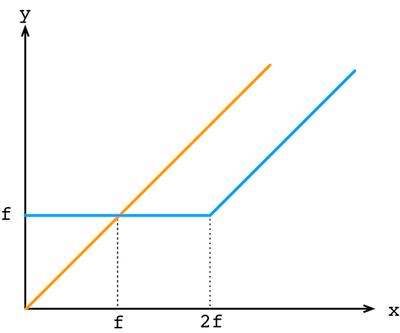
\includegraphics[height=6cm]{images/fee-model.png}
\label{fig: Loopringrotocol}
\end{figurehere}
\end{center}

where: $f$ is the LRCfee, $x$ is the margin split, and $y$ is the miner's income.
If $f$ is the LRC fee and $x$ the margin split, then the miner's income $y$ is $y = max(f, x-f)$, and we get the blue line.
If the specified LRC fee for the order is 0, the equation is $y = max(0, x - 0)$ that simplifies to $y = x$, and we get the orange line.
This has the following consequences: if the margin split is 0, the miners will choose the flat LRC fee and are still incentivized. If the LRC fee is 0, this is the orange line, the income is based on a general model. When the margin split income gets bigger than twice the LRC fee, only then will the miner choose the margin split.
It should be noted that if the LRC fee is non-zero, no matter which option the miner chooses, there will always be a transfer of LRC between the miner and the order's sender, either by sending back the LRC surplus fee or by paying the sender the LRC fee to take the margin split.
The current fee model is still open for discussion.

\subsection{Emitted Events}
This section will describe the set of events that the LSC emits. These events exist to allow the relay/order browsers and other elements that need an update of their order books to receive the information as quickly as possible.
A list of the emitted events: \textbf{OrderCancelled}, \textbf{OrderFilled}, \textbf{RingMined}.

\subsection{Fraud and Attack Protections}
\subsubsection{Ring Filch}
An attacker could monitor all unconfirmed Rings and broadcast the same Rings with his own digital signature. We call this Ring Filch. In order to prevent Ring Filch, Loopring allows miners to use two steps in order to submit their Rings:
\begin{itemize}
	\item Submit the Ring’s hash and wait for confirmation; or
	\item Submit the Ring themselves.
\end{itemize}
This protection is valid for a \textbf{ttl} time specified in the LSC. After that duration, if the ring has not been submitted, another miner can claim it.
\subsubsection{Denial of Service}
We allow nodes to selectively handle orders by setting their own criteria, and they may choose to hide or reveal it. Therefore, we do not see denial of service as a form of unethical behavior.
\subsubsection{Massive Tiny Order Attack}
A user could send a large amount of tiny orders to attack the Loopring nodes. However, since we allow nodes to reject orders based on their own criteria, most of these orders will be rejected because they do not yield satisfying profit when matched. This makes a massive tiny order attack not feasible.

\subsubsection{Insufficient Balance}
Malicious users may sign and spread out orders, whose value inside the order is not zero but whose address actually has zero balance. Nodes could monitor and notice that some orders actual balance is zero, update these orders states accordingly. and then discard them.
Nodes do have to spend time to update an order’s status, but nodes can also choose to minimize the effort by, for example, blacklisting addresses and drop related orders.
\end{document}
